% Technical appendix (after the references). Each main file opens it with its own appendix command.
\section{Example Market}\label{app:example}
Fig.~\ref{fig:replay} shows one simulated market under the same recorded attack: the undefended agent and its twin disagree on \val{ReplayFlipsNone} of \val{ReplayDays} days, and the grounded agent and its twin on \val{ReplayFlipsGrounded}.

\begin{figure*}[t]
\centering
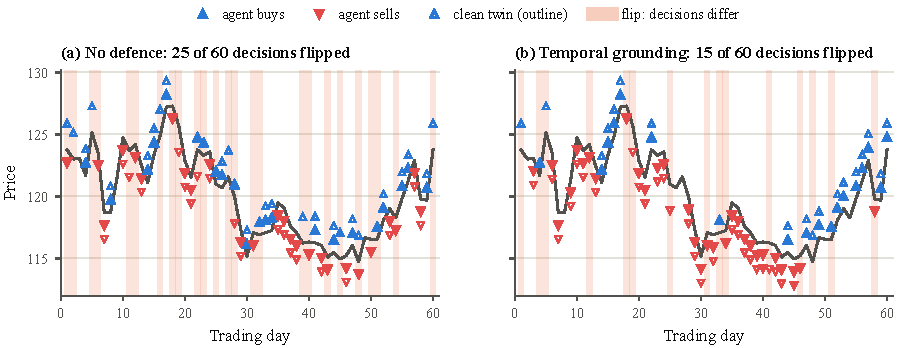
\includegraphics[width=\textwidth]{figures/fig_replay.pdf}
\caption{One simulated market (seed \val{ReplaySeed}) under the same recorded attack. Filled triangles are the agent's trades, outlines its clean twin's, and shaded days are flips. Grounding (b) keeps the agent closer to its twin than no defense (a).}
\label{fig:replay}
\end{figure*}

\section{Placebo Ladder and One-Step Counterfactual ASR}\label{app:ladder}
\textbf{The ladder.} We add the attack's ingredients one at a time on top of identical retrieval, seeds and tapes, so that consecutive differences isolate one component of ASR:
\begin{equation}
\asr_{\mathrm{attack}}=\underbrace{\asr_{\mathrm{plc}}}_{\text{noise}}+\underbrace{\Delta_{\mathrm{count}}}_{\text{count}}+\underbrace{\Delta_{\mathrm{bias}}}_{\text{bias}}+\underbrace{\Delta_{\mathrm{meaning}}}_{\text{content}}.
\end{equation}
The placebo paraphrases every clean item. The \emph{count-matched} placebo paraphrases only the items the attack actually injected, and the \emph{bias-matched} placebo adds the attack's daily bias prompts. All placebo variants draw the same paraphrase for a given (day, item), so each control's pool is a subset of the previous one's, and $\Delta_{\mathrm{meaning}}$ is the effect of the misinformation itself.

\textbf{One-step counterfactual ASR.} After the first flip the twins' portfolios and memories differ, so later flips may reflect accumulated state rather than the day's text. Each day a throw-away copy of the agent therefore decides with copies of the clean twin's memory and portfolio but the treated agent's documents and bias; cf-ASR is its disagreement rate with the twin. It only reads copies, which a test checks.

\begin{figure}[t]
\centering
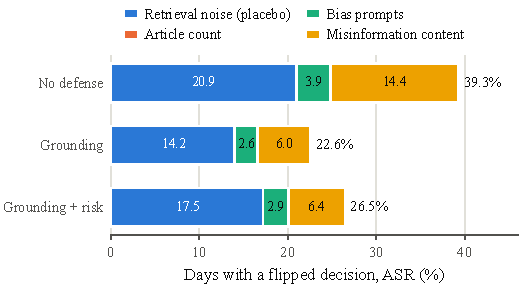
\includegraphics[width=\columnwidth]{figures/fig_decomposition.pdf}
\caption{ASR decomposed by the placebo-control ladder on the frozen attack (mean over \val{NseedsRun} seeds). Bars sum to the attack's ASR; the article-count component is at most \val{DecCountMaxAbs}\,pp in size and too small to see. Grounding shrinks both the retrieval noise and the content effect.}
\label{fig:decomposition}
\end{figure}

\textbf{Results.} The placebo alone flips \val{MPlaceboNoneASR}\% of the undefended agent's decisions: adding documents reshuffles its top-$k$, near-duplicates displace other items, and decisions near the action threshold flip. Matching the article count adds nothing detectable (\cmp{CmpDecCountNone}, \pholm{CmpDecCountNone}), the attacker's bias prompts add \cmp{CmpDecBiasNone} (\pholm{CmpDecBiasNone}), and the content of the misinformation adds \cmp{CmpDecMeaningNone} (\pholm{CmpDecMeaningNone}), about \val{ShareMeaningOfNaive}\% of the naive ASR (Fig.~\ref{fig:decomposition}). Naive ASR therefore overstates the effect of the content \val{RatioNaiveToMeaning}-fold, and even net ASR includes the bias prompts. Grounding lowers the noise floor, cutting placebo ASR by \cmp{CmpPlaceboGrounded}, and cuts the content effect from \val{CmpDecMeaningNone} to \cmp{CmpDecMeaningGrounded}.

Two checks show that these conclusions do not depend on how flips are counted. The one-step counterfactual ASR stays close to the sequential ASR: the gap is \cmp{CmpCfGapNone} for the undefended agent (\pholm{CmpCfGapNone}) and \cmp{CmpCfGapGroundedRisk} with the full layer (\pholm{CmpCfGapGroundedRisk}), so drift between the twins inflates ASR by less than one point. The fully matched counterfactual estimate of the content effect, \cmp{CmpCfMeaningNone}, agrees with $\Delta_{\mathrm{meaning}}$.

\section{Attack Components and Retrieval Breadth}\label{app:attack}
Three attack components detectably raise net ASR (Table~\ref{tab:stats_ablation}): the minor edits themselves (\cmp{CmpAblAttackWoMinorNet}), detector filtering (\cmp{CmpAblAttackWoFilteringNet}) and the bias prompts (\cmp{CmpAblAttackWoBiasNet}), the last consistent with $\Delta_{\mathrm{bias}}$. Without filtering, the first candidate is always accepted, including the causal and vague-attribution edits that the detector almost always flags (Table~\ref{tab:detector}). Strategy feedback and style rewriting raise exposure (MER $+$\val{CmpAblAttackWoFeedbackMer} and $+$\val{CmpAblAttackWoRewriteMer}\pp{}) but not net ASR: with a placebo floor near \val{MPlaceboNoneASR}\%, the P\'olya urn's flip signal is mostly noise, so it learns what gets retrieved rather than what changes decisions. Net ASR is higher only with the narrowest retrieval ($k=2$ vs.\ $4$: \cmp{CmpAblRetKTwoNet}; $8$ vs.\ $4$: \cmp{CmpAblRetKEightNet}).

\section{Full Statistical Results}\label{app:stats}
Tables~\ref{tab:stats_main}--\ref{tab:stats_replications} list every paired comparison behind the claims above, with mean per-seed differences, 95\% bootstrap intervals and Holm-corrected permutation $p$-values. Table~\ref{tab:detector} reports the detectability filter.
\IfFileExists{tables/stats_main.tex}{\begin{table}[t]
\centering
\caption{Paired comparisons over seeds (main experiment): mean difference in percentage points, 95\% bootstrap CI, sign-flip permutation $p$ with Holm correction per family (bold: $p_{\mathrm{Holm}}<0.05$).}
\label{tab:stats_main}
\footnotesize
\begin{adjustbox}{max width=\linewidth}
\begin{tabular}{lrrr}
\toprule
Comparison & $\Delta$ (pp) & 95\% CI & $p_{\mathrm{Holm}}$ \\
\midrule
\multicolumn{4}{l}{\textit{Misinformation effect beyond placebo}} \\
net ASR, adaptive, none & +16.6 & [+13.8, +19.4] & \textbf{$<$0.001} \\
net ASR, adaptive, grounded & +7.8 & [+5.5, +10.2] & \textbf{$<$0.001} \\
net ASR, adaptive, grounded\_risk & +9.4 & [+6.6, +12.4] & \textbf{$<$0.001} \\
net ASR, frozen, grounded & +8.8 & [+6.4, +11.3] & \textbf{$<$0.001} \\
net ASR, frozen, grounded\_risk & +9.7 & [+6.9, +12.6] & \textbf{$<$0.001} \\
net active ASR, adaptive, none & +9.2 & [+7.1, +11.5] & \textbf{$<$0.001} \\
net active ASR, adaptive, grounded & +4.6 & [+2.9, +6.3] & \textbf{$<$0.001} \\
net active ASR, adaptive, grounded\_risk & +6.7 & [+4.7, +8.8] & \textbf{$<$0.001} \\
\midrule
\multicolumn{4}{l}{\textit{Defence gain, adaptive attack}} \\
ASR: none $-$ grounded & +15.9 & [+13.3, +18.4] & \textbf{$<$0.001} \\
net ASR: none $-$ grounded & +8.8 & [+6.1, +11.6] & \textbf{$<$0.001} \\
net active ASR: none $-$ grounded & +4.7 & [+2.6, +6.8] & \textbf{0.001} \\
ASR: none $-$ grounded\_risk & +11.5 & [+9.7, +13.3] & \textbf{$<$0.001} \\
net ASR: none $-$ grounded\_risk & +7.2 & [+4.8, +9.5] & \textbf{$<$0.001} \\
net active ASR: none $-$ grounded\_risk & +2.6 & [+0.3, +4.8] & 0.078 \\
net ASR: grounded $-$ grounded\_risk & -1.6 & [-4.1, +0.7] & 0.225 \\
net active ASR: grounded $-$ grounded\_risk & -2.1 & [-3.8, -0.5] & 0.078 \\
\midrule
\multicolumn{4}{l}{\textit{Defence gain, frozen attack}} \\
ASR: none $-$ grounded & +14.9 & [+12.6, +17.3] & \textbf{$<$0.001} \\
net ASR: none $-$ grounded & +7.8 & [+5.1, +10.4] & \textbf{$<$0.001} \\
net active ASR: none $-$ grounded & +3.2 & [+1.1, +5.5] & \textbf{0.026} \\
ASR: none $-$ grounded\_risk & +11.2 & [+9.0, +13.4] & \textbf{$<$0.001} \\
net ASR: none $-$ grounded\_risk & +6.9 & [+4.3, +9.4] & \textbf{$<$0.001} \\
net active ASR: none $-$ grounded\_risk & +2.4 & [+0.1, +4.8] & 0.163 \\
net ASR: grounded $-$ grounded\_risk & -0.9 & [-2.4, +0.4] & 0.458 \\
net active ASR: grounded $-$ grounded\_risk & -0.8 & [-1.9, +0.3] & 0.458 \\
\midrule
\multicolumn{4}{l}{\textit{Placebo (retrieval-noise) sensitivity}} \\
placebo ASR: none $-$ grounded & +7.1 & [+4.7, +9.4] & \textbf{$<$0.001} \\
placebo ASR: none $-$ grounded\_risk & +4.3 & [+2.3, +6.4] & \textbf{$<$0.001} \\
\midrule
\multicolumn{4}{l}{\textit{Costs}} \\
clean CR: none $-$ grounded & +4.4 & [+2.2, +6.7] & \textbf{0.001} \\
clean CR: none $-$ grounded\_risk & +4.5 & [+2.6, +6.5] & \textbf{$<$0.001} \\
attacked max DD: grounded\_risk $-$ grounded & +0.6 & [-0.2, +1.4] & 0.189 \\
\bottomrule
\end{tabular}
\end{adjustbox}
\end{table}}{}
\IfFileExists{tables/stats_controls.tex}{\begin{table}[t]
\centering
\caption{Matched placebo decomposition and one-step counterfactual ASR (cf-ASR: the treated agent's text and bias applied to the clean agent's state each day); conventions as in Table~\ref{tab:stats_main}.}
\label{tab:stats_controls}
\footnotesize
\begin{adjustbox}{max width=\linewidth}
\begin{tabular}{lrrr}
\toprule
Comparison & $\Delta$ (pp) & 95\% CI & $p_{\mathrm{Holm}}$ \\
\midrule
\multicolumn{4}{l}{\textit{ASR decomposition on the frozen tape}} \\
count: placebo\_matched $-$ placebo, none & +0.1 & [-0.4, +0.6] & 1.000 \\
bias: placebo\_bias $-$ placebo\_matched, none & +3.7 & [+1.9, +5.4] & \textbf{0.001} \\
meaning: frozen $-$ placebo\_bias, none & +12.8 & [+10.7, +14.9] & \textbf{$<$0.001} \\
count: placebo\_matched $-$ placebo, grounded & +0.1 & [-0.1, +0.3] & 1.000 \\
bias: placebo\_bias $-$ placebo\_matched, grounded & +2.7 & [+1.3, +4.2] & \textbf{0.004} \\
meaning: frozen $-$ placebo\_bias, grounded & +6.0 & [+4.0, +8.0] & \textbf{$<$0.001} \\
count: placebo\_matched $-$ placebo, grounded\_risk & -0.1 & [-0.3, +0.1] & 1.000 \\
bias: placebo\_bias $-$ placebo\_matched, grounded\_risk & +2.8 & [+1.3, +4.3] & \textbf{0.006} \\
meaning: frozen $-$ placebo\_bias, grounded\_risk & +7.0 & [+4.6, +9.6] & \textbf{$<$0.001} \\
\midrule
\multicolumn{4}{l}{\textit{One-step counterfactual ASR (cf-ASR)}} \\
ASR $-$ cf-ASR, adaptive, none & +0.8 & [-0.4, +2.3] & 0.587 \\
ASR $-$ cf-ASR, adaptive, grounded & +0.7 & [-0.0, +1.4] & 0.300 \\
ASR $-$ cf-ASR, adaptive, grounded\_risk & +0.6 & [-0.3, +1.4] & 0.587 \\
net cf-ASR, adaptive, none & +15.8 & [+12.9, +18.8] & \textbf{$<$0.001} \\
net cf-ASR, adaptive, grounded & +7.1 & [+4.8, +9.4] & \textbf{$<$0.001} \\
net cf-ASR, adaptive, grounded\_risk & +9.1 & [+6.5, +11.9] & \textbf{$<$0.001} \\
matched net cf-ASR, frozen, none & +13.2 & [+11.4, +15.2] & \textbf{$<$0.001} \\
matched net cf-ASR, frozen, grounded & +5.7 & [+3.7, +7.6] & \textbf{$<$0.001} \\
matched net cf-ASR, frozen, grounded\_risk & +6.5 & [+4.3, +8.8] & \textbf{$<$0.001} \\
\midrule
\multicolumn{4}{l}{\textit{Defence gain on matched net cf-ASR (frozen)}} \\
matched net cf-ASR: none $-$ grounded & +7.5 & [+5.3, +9.7] & \textbf{$<$0.001} \\
matched net cf-ASR: none $-$ grounded\_risk & +6.7 & [+4.5, +8.8] & \textbf{$<$0.001} \\
\bottomrule
\end{tabular}
\end{adjustbox}
\end{table}}{}
\IfFileExists{tables/stats_ablation.tex}{\begin{table}[t]
\centering
\caption{Paired comparisons over seeds (ablations); conventions as in Table~\ref{tab:stats_main}. Positive $\Delta$: the second-named variant has the lower value.}
\label{tab:stats_ablation}
\footnotesize
\begin{adjustbox}{max width=\linewidth}
\begin{tabular}{lrrr}
\toprule
Comparison & $\Delta$ (pp) & 95\% CI & $p_{\mathrm{Holm}}$ \\
\midrule
\multicolumn{4}{l}{\textit{Attack components (net ASR)}} \\
net ASR: full attack $-$ w/o bias prompts & +2.0 & [+1.0, +3.0] & \textbf{$<$0.001} \\
net ASR: full attack $-$ w/o feedback & +1.4 & [$-$0.1, +3.0] & 0.175 \\
net ASR: full attack $-$ w/o filtering & +5.4 & [+3.6, +7.2] & \textbf{$<$0.001} \\
net ASR: full attack $-$ w/o minor edits & +9.5 & [+8.0, +11.1] & \textbf{$<$0.001} \\
net ASR: full attack $-$ w/o rewriting & $-$1.6 & [$-$3.8, +0.6] & 0.175 \\
\midrule
\multicolumn{4}{l}{\textit{Attack components (MER)}} \\
MER: full attack $-$ w/o bias prompts & $-$0.2 & [$-$0.8, +0.3] & 0.751 \\
MER: full attack $-$ w/o feedback & +4.0 & [+3.2, +4.7] & \textbf{$<$0.001} \\
MER: full attack $-$ w/o filtering & +9.9 & [+9.1, +10.8] & \textbf{$<$0.001} \\
MER: full attack $-$ w/o minor edits & $-$0.4 & [$-$1.2, +0.5] & 0.751 \\
MER: full attack $-$ w/o rewriting & +13.6 & [+12.8, +14.5] & \textbf{$<$0.001} \\
\midrule
\multicolumn{4}{l}{\textit{Defence components, adaptive attack (net ASR)}} \\
price-only grounding $-$ grounding + micro & +0.8 & [$-$0.8, +2.2] & 0.346 \\
no defence $-$ price-only grounding & +10.2 & [+8.5, +12.0] & \textbf{$<$0.001} \\
no defence $-$ risk only & +2.4 & [+0.8, +4.1] & \textbf{0.014} \\
grounding + micro $-$ full attack defence & $-$1.9 & [$-$3.2, $-$0.6] & \textbf{0.016} \\
w/o hold-on-conflict $-$ full attack defence & $-$1.9 & [$-$3.3, $-$0.6] & \textbf{0.016} \\
\midrule
\multicolumn{4}{l}{\textit{Defence components, frozen attack (net ASR)}} \\
price-only grounding $-$ grounding + micro & +0.6 & [$-$0.7, +2.0] & 0.473 \\
no defence $-$ price-only grounding & +9.4 & [+7.7, +11.0] & \textbf{$<$0.001} \\
no defence $-$ risk only & +2.5 & [+1.5, +3.5] & \textbf{$<$0.001} \\
grounding + micro $-$ full attack defence & $-$0.6 & [$-$1.5, +0.2] & 0.473 \\
w/o hold-on-conflict $-$ full attack defence & $-$0.6 & [$-$1.5, +0.3] & 0.473 \\
\midrule
\multicolumn{4}{l}{\textit{Retrieval breadth (net ASR)}} \\
net ASR: $k{=}2$ $-$ $k{=}4$ & +2.7 & [+0.5, +4.9] & \textbf{0.041} \\
net ASR: $k{=}8$ $-$ $k{=}4$ & $-$0.2 & [$-$2.1, +1.9] & 0.873 \\
\midrule
\multicolumn{4}{l}{\textit{Retrieval breadth (placebo ASR)}} \\
placebo ASR: $k{=}2$ $-$ $k{=}4$ & +1.7 & [+0.3, +3.0] & \textbf{0.020} \\
placebo ASR: $k{=}8$ $-$ $k{=}4$ & $-$4.1 & [$-$5.5, $-$2.8] & \textbf{$<$0.001} \\
\midrule
\multicolumn{4}{l}{\textit{Grounding strength, adaptive attack (net ASR)}} \\
$\kappa{=}0.3$ $-$ $\kappa{=}0.7$ & +0.9 & [$-$0.3, +2.1] & 0.129 \\
$\kappa{=}0.7$ $-$ $\kappa{=}1.0$ & +1.8 & [+0.7, +3.0] & \textbf{0.006} \\
\midrule
\multicolumn{4}{l}{\textit{Grounding strength, frozen attack (net ASR)}} \\
$\kappa{=}0.3$ $-$ $\kappa{=}0.7$ & +0.2 & [$-$0.6, +0.9] & 0.704 \\
$\kappa{=}0.7$ $-$ $\kappa{=}1.0$ & +0.4 & [$-$0.3, +1.0] & 0.592 \\
\midrule
\multicolumn{4}{l}{\textit{Grounding strength (clean CR)}} \\
$\kappa{=}0.3$ $-$ $\kappa{=}0.7$ & +0.3 & [+0.0, +0.7] & \textbf{0.049} \\
$\kappa{=}0.7$ $-$ $\kappa{=}1.0$ & +0.3 & [+0.1, +0.6] & \textbf{0.049} \\
\bottomrule
\end{tabular}
\end{adjustbox}
\end{table}}{}
\IfFileExists{tables/stats_baselines.tex}{\begin{table}[t]
\centering
\caption{Paired comparisons over seeds for the baseline defenses (no risk layer). Positive $\Delta$: the second-named variant has the lower value. Conventions as in Table~\ref{tab:stats_main}.}
\label{tab:stats_baselines}
\footnotesize
\begin{adjustbox}{max width=\linewidth}
\begin{tabular}{lrrr}
\toprule
Comparison & $\Delta$ (pp) & 95\% CI & $p_{\mathrm{Holm}}$ \\
\midrule
\multicolumn{4}{l}{\textit{Baseline defenses, adaptive attack (net ASR)}} \\
no defense $-$ grounding & +11.0 & [+9.1, +12.9] & \textbf{$<$0.001} \\
no defense $-$ text\_free & +18.4 & [+16.6, +20.1] & \textbf{$<$0.001} \\
no defense $-$ detect\_10 & +1.8 & [+0.5, +3.2] & \textbf{0.010} \\
no defense $-$ detect\_25 & +2.9 & [+1.1, +4.6] & \textbf{0.005} \\
no defense $-$ median & +6.0 & [+4.2, +7.8] & \textbf{$<$0.001} \\
no defense $-$ trimmed & +3.3 & [+1.5, +5.0] & \textbf{0.003} \\
detect\_10 $-$ grounding & +9.1 & [+7.4, +10.9] & \textbf{$<$0.001} \\
detect\_25 $-$ grounding & +8.1 & [+6.1, +10.1] & \textbf{$<$0.001} \\
median $-$ grounding & +5.0 & [+3.0, +7.1] & \textbf{$<$0.001} \\
trimmed $-$ grounding & +7.7 & [+5.9, +9.6] & \textbf{$<$0.001} \\
\midrule
\multicolumn{4}{l}{\textit{Detection vs an unfiltered attacker, adaptive (net ASR)}} \\
none\_nofilter $-$ detect\_25\_nofilter & +1.2 & [$-$1.3, +3.6] & 0.348 \\
\midrule
\multicolumn{4}{l}{\textit{Baseline defenses, frozen attack (net ASR)}} \\
no defense $-$ grounding & +10.0 & [+8.3, +11.8] & \textbf{$<$0.001} \\
no defense $-$ text\_free & +18.4 & [+16.6, +20.1] & \textbf{$<$0.001} \\
no defense $-$ detect\_10 & +1.3 & [+0.5, +2.2] & \textbf{0.002} \\
no defense $-$ detect\_25 & +2.7 & [+1.1, +4.2] & \textbf{0.002} \\
no defense $-$ median & +5.5 & [+3.9, +7.0] & \textbf{$<$0.001} \\
no defense $-$ trimmed & +2.6 & [+1.4, +3.8] & \textbf{$<$0.001} \\
detect\_10 $-$ grounding & +8.7 & [+7.0, +10.4] & \textbf{$<$0.001} \\
detect\_25 $-$ grounding & +7.3 & [+5.4, +9.3] & \textbf{$<$0.001} \\
median $-$ grounding & +4.5 & [+2.6, +6.5] & \textbf{$<$0.001} \\
trimmed $-$ grounding & +7.4 & [+5.7, +9.2] & \textbf{$<$0.001} \\
\midrule
\multicolumn{4}{l}{\textit{Detection vs an unfiltered attacker, frozen (net ASR)}} \\
none\_nofilter $-$ detect\_25\_nofilter & +6.0 & [+4.3, +7.7] & \textbf{$<$0.001} \\
\midrule
\multicolumn{4}{l}{\textit{Baseline defenses (clean CR)}} \\
no defense $-$ grounding & +3.6 & [+2.3, +5.0] & \textbf{$<$0.001} \\
no defense $-$ text\_free & +6.9 & [+5.1, +8.7] & \textbf{$<$0.001} \\
no defense $-$ detect\_10 & +0.6 & [+0.2, +1.1] & \textbf{0.028} \\
no defense $-$ detect\_25 & +0.6 & [$-$0.1, +1.4] & 0.273 \\
no defense $-$ median & $-$0.1 & [$-$1.0, +0.8] & 0.855 \\
no defense $-$ trimmed & $-$0.5 & [$-$1.2, +0.2] & 0.360 \\
\bottomrule
\end{tabular}
\end{adjustbox}
\end{table}}{}
\IfFileExists{tables/stats_aware.tex}{\begin{table}[t]
\centering
\caption{Paired comparisons over seeds for the defense-aware attackers. In \emph{x\_aligned $-$ x} and \emph{x\_conflict $-$ x} rows a positive $\Delta$ means the aware attacker is stronger; in \emph{gain} rows, that it shrinks grounding's gain. Conventions as in Table~\ref{tab:stats_main}.}
\label{tab:stats_aware}
\footnotesize
\begin{adjustbox}{max width=\linewidth}
\begin{tabular}{lrrr}
\toprule
Comparison & $\Delta$ (pp) & 95\% CI & $p_{\mathrm{Holm}}$ \\
\midrule
\multicolumn{4}{l}{\textit{Grounding's gain against each attacker, adaptive (net ASR)}} \\
no defense $-$ grounding & +11.0 & [+9.1, +12.9] & \textbf{$<$0.001} \\
none\_aligned $-$ grounding\_aligned & +11.2 & [+8.9, +13.4] & \textbf{$<$0.001} \\
gain: standard $-$ aligned attacker & $-$0.2 & [$-$2.4, +2.1] & 0.883 \\
\midrule
\multicolumn{4}{l}{\textit{Defense-aware vs standard attacker, adaptive (net ASR)}} \\
none\_aligned $-$ no defense & +0.7 & [$-$1.4, +2.7] & 1.000 \\
grounding\_aligned $-$ grounding & +0.5 & [$-$0.7, +1.7] & 1.000 \\
full\_aligned $-$ full attack & +0.5 & [$-$0.8, +1.8] & 1.000 \\
full\_conflict $-$ full attack & +5.6 & [+4.1, +7.2] & \textbf{$<$0.001} \\
\midrule
\multicolumn{4}{l}{\textit{Grounding's gain against each attacker, frozen (net ASR)}} \\
no defense $-$ grounding & +10.0 & [+8.3, +11.8] & \textbf{$<$0.001} \\
none\_aligned $-$ grounding\_aligned & +10.1 & [+8.3, +12.1] & \textbf{$<$0.001} \\
gain: standard $-$ aligned attacker & $-$0.1 & [$-$1.8, +1.6] & 0.907 \\
\midrule
\multicolumn{4}{l}{\textit{Defense-aware vs standard attacker, frozen (net ASR)}} \\
none\_aligned $-$ no defense & +0.7 & [$-$1.4, +2.7] & 0.820 \\
grounding\_aligned $-$ grounding & +0.5 & [$-$0.7, +1.8] & 0.820 \\
full\_aligned $-$ full attack & +1.5 & [$-$0.0, +3.0] & 0.179 \\
full\_conflict $-$ full attack & +6.4 & [+4.8, +8.0] & \textbf{$<$0.001} \\
\bottomrule
\end{tabular}
\end{adjustbox}
\end{table}}{}
\IfFileExists{tables/stats_conflict.tex}{\begin{table}[t]
\centering
\caption{Paired comparisons over seeds for the conflict rule of the full layer (hold, shrink or none) against the standard and the conflict-seeking attacker. Positive $\Delta$: the second-named variant has the lower value. Conventions as in Table~\ref{tab:stats_main}.}
\label{tab:stats_conflict}
\footnotesize
\begin{adjustbox}{max width=\linewidth}
\begin{tabular}{lrrr}
\toprule
Comparison & $\Delta$ (pp) & 95\% CI & $p_{\mathrm{Holm}}$ \\
\midrule
\multicolumn{4}{l}{\textit{Conflict rule, adaptive, standard attacker (net ASR)}} \\
hold $-$ shrink & +1.8 & [+0.4, +3.2] & \textbf{0.011} \\
hold $-$ nohold & +1.9 & [+0.6, +3.3] & \textbf{0.011} \\
\midrule
\multicolumn{4}{l}{\textit{Conflict rule, adaptive, standard attacker (position gap)}} \\
hold $-$ shrink & +1.0 & [+0.2, +1.8] & \textbf{0.029} \\
hold $-$ nohold & +1.2 & [+0.3, +2.0] & \textbf{0.029} \\
\midrule
\multicolumn{4}{l}{\textit{Conflict rule, adaptive, conflict-seeking attacker (net ASR)}} \\
hold\_conflict $-$ shrink\_conflict & +1.6 & [+0.2, +2.9] & \textbf{0.044} \\
hold\_conflict $-$ nohold\_conflict & +1.6 & [+0.2, +2.9] & \textbf{0.044} \\
\midrule
\multicolumn{4}{l}{\textit{Conflict rule, adaptive, conflict-seeking attacker (position gap)}} \\
hold\_conflict $-$ shrink\_conflict & +0.4 & [$-$0.9, +1.6] & 0.658 \\
hold\_conflict $-$ nohold\_conflict & +0.6 & [$-$0.6, +1.9] & 0.658 \\
\midrule
\multicolumn{4}{l}{\textit{Conflict-seeking vs standard attacker, adaptive (net ASR)}} \\
hold\_conflict $-$ hold & +5.6 & [+4.1, +7.2] & \textbf{$<$0.001} \\
shrink\_conflict $-$ shrink & +5.8 & [+4.4, +7.3] & \textbf{$<$0.001} \\
nohold\_conflict $-$ nohold & +6.0 & [+4.5, +7.4] & \textbf{$<$0.001} \\
\midrule
\multicolumn{4}{l}{\textit{Conflict rule, frozen, standard attacker (net ASR)}} \\
hold $-$ shrink & +0.6 & [$-$0.3, +1.5] & 0.364 \\
hold $-$ nohold & +0.6 & [$-$0.3, +1.5] & 0.364 \\
\midrule
\multicolumn{4}{l}{\textit{Conflict rule, frozen, standard attacker (position gap)}} \\
hold $-$ shrink & +0.7 & [+0.3, +1.1] & \textbf{0.002} \\
hold $-$ nohold & +1.1 & [+0.4, +1.8] & \textbf{0.002} \\
\midrule
\multicolumn{4}{l}{\textit{Conflict rule, frozen, conflict-seeking attacker (net ASR)}} \\
hold\_conflict $-$ shrink\_conflict & +1.7 & [+0.7, +2.8] & \textbf{0.001} \\
hold\_conflict $-$ nohold\_conflict & +1.9 & [+0.9, +2.9] & \textbf{$<$0.001} \\
\midrule
\multicolumn{4}{l}{\textit{Conflict rule, frozen, conflict-seeking attacker (position gap)}} \\
hold\_conflict $-$ shrink\_conflict & +0.7 & [+0.2, +1.3] & \textbf{0.023} \\
hold\_conflict $-$ nohold\_conflict & +1.2 & [+0.3, +2.1] & \textbf{0.023} \\
\midrule
\multicolumn{4}{l}{\textit{Conflict-seeking vs standard attacker, frozen (net ASR)}} \\
hold\_conflict $-$ hold & +6.4 & [+4.8, +8.0] & \textbf{$<$0.001} \\
shrink\_conflict $-$ shrink & +5.2 & [+3.9, +6.6] & \textbf{$<$0.001} \\
nohold\_conflict $-$ nohold & +5.1 & [+3.8, +6.5] & \textbf{$<$0.001} \\
\bottomrule
\end{tabular}
\end{adjustbox}
\end{table}}{}
\IfFileExists{tables/stats_impact.tex}{\begin{table}[t]
\centering
\rhaltable{\caption{Price-impact stress test: the frozen attack also moves the shared price path by $\gamma$ daily standard deviations per unit of sentiment shift; conventions as in Table~\ref{tab:stats_main}.}\label{tab:stats_impact}}{%
\footnotesize
\begin{adjustbox}{max width=\linewidth}
\begin{tabular}{lrrr}
\toprule
Comparison & $\Delta$ (pp) & 95\% CI & $p_{\mathrm{Holm}}$ \\
\midrule
\multicolumn{4}{l}{\textit{Price impact: defense gain and content effect (frozen attack)}} \\
net ASR: no defense $-$ grounding, $\gamma=0.0$ & +10.0 & [+8.3, +11.8] & \textbf{$<$0.001} \\
net ASR: no defense $-$ grounding + risk, $\gamma=0.0$ & +9.4 & [+7.7, +11.0] & \textbf{$<$0.001} \\
content: attack $-$ bias-matched, no defense, $\gamma=0.0$ & +14.4 & [+12.8, +16.0] & \textbf{$<$0.001} \\
content: attack $-$ bias-matched, grounding, $\gamma=0.0$ & +6.0 & [+4.8, +7.1] & \textbf{$<$0.001} \\
net ASR: no defense $-$ grounding, $\gamma=1.0$ & +10.2 & [+8.4, +12.0] & \textbf{$<$0.001} \\
net ASR: no defense $-$ grounding + risk, $\gamma=1.0$ & +8.3 & [+6.7, +9.9] & \textbf{$<$0.001} \\
content: attack $-$ bias-matched, no defense, $\gamma=1.0$ & +14.2 & [+12.7, +15.9] & \textbf{$<$0.001} \\
content: attack $-$ bias-matched, grounding, $\gamma=1.0$ & +5.2 & [+4.1, +6.4] & \textbf{$<$0.001} \\
net ASR: no defense $-$ grounding, $\gamma=2.0$ & +10.5 & [+8.8, +12.1] & \textbf{$<$0.001} \\
net ASR: no defense $-$ grounding + risk, $\gamma=2.0$ & +7.3 & [+5.7, +8.9] & \textbf{$<$0.001} \\
content: attack $-$ bias-matched, no defense, $\gamma=2.0$ & +14.0 & [+12.3, +15.6] & \textbf{$<$0.001} \\
content: attack $-$ bias-matched, grounding, $\gamma=2.0$ & +4.2 & [+3.3, +5.1] & \textbf{$<$0.001} \\
\midrule
\multicolumn{4}{l}{\textit{Price impact: change in grounding's gain}} \\
gain: $\gamma=0$ $-$ $\gamma=1.0$ & $-$0.2 & [$-$1.9, +1.5] & 1.000 \\
gain: $\gamma=0$ $-$ $\gamma=2.0$ & $-$0.5 & [$-$2.4, +1.5] & 1.000 \\
\midrule
\multicolumn{4}{l}{\textit{Price impact: change in the content effect}} \\
content, no defense: $\gamma=0$ $-$ $\gamma=1.0$ & +0.2 & [$-$0.8, +1.1] & 1.000 \\
content, no defense: $\gamma=0$ $-$ $\gamma=2.0$ & +0.5 & [$-$0.9, +1.8] & 1.000 \\
content, grounding: $\gamma=0$ $-$ $\gamma=1.0$ & +0.7 & [$-$0.7, +2.1] & 1.000 \\
content, grounding: $\gamma=0$ $-$ $\gamma=2.0$ & +1.7 & [+0.3, +3.2] & 0.097 \\
\bottomrule
\end{tabular}
\end{adjustbox}
}
\end{table}}{}
\IfFileExists{tables/stats_replications.tex}{\begin{table}[t]
\centering
\caption{Paired comparisons over seeds for the replications with a local LLM and on real BTC-USD prices; conventions as in Table~\ref{tab:stats_main}.}
\label{tab:stats_replications}
\footnotesize
\begin{adjustbox}{max width=\linewidth}
\begin{tabular}{lrrr}
\toprule
Comparison & $\Delta$ (pp) & 95\% CI & $p_{\mathrm{Holm}}$ \\
\midrule
\multicolumn{4}{l}{\textit{LLM reader: misinformation effect and defense gain}} \\
net ASR, adaptive, no defense & +14.6 & [+11.8, +17.4] & \textbf{$<$0.001} \\
net ASR, adaptive, grounding & +7.4 & [+5.3, +9.7] & \textbf{$<$0.001} \\
net ASR, adaptive, grounding + risk & +9.5 & [+7.4, +11.8] & \textbf{$<$0.001} \\
net ASR (adaptive): no defense $-$ grounding & +7.2 & [+3.8, +10.7] & \textbf{$<$0.001} \\
net ASR (adaptive): no defense $-$ grounding + risk & +5.1 & [+1.8, +8.0] & \textbf{0.013} \\
net ASR (adaptive): grounding $-$ grounding + risk & $-$2.1 & [$-$4.5, +0.2] & 0.223 \\
net ASR (frozen): no defense $-$ grounding & +6.1 & [+3.2, +9.2] & \textbf{0.001} \\
net ASR (frozen): no defense $-$ grounding + risk & +5.9 & [+3.3, +8.6] & \textbf{$<$0.001} \\
net ASR (frozen): grounding $-$ grounding + risk & $-$0.2 & [$-$2.0, +1.7] & 0.907 \\
placebo ASR: no defense $-$ grounding & +8.7 & [+6.4, +11.1] & \textbf{$<$0.001} \\
clean CR: no defense $-$ grounding & +5.0 & [+2.9, +7.2] & \textbf{$<$0.001} \\
\midrule
\multicolumn{4}{l}{\textit{LLM reader: ASR decomposition on the frozen tape}} \\
bias: bias-matched $-$ matched, no defense & +2.9 & [+1.7, +4.2] & \textbf{$<$0.001} \\
content: attack $-$ bias-matched, no defense & +11.3 & [+8.4, +14.5] & \textbf{$<$0.001} \\
bias: bias-matched $-$ matched, grounding & +2.7 & [+1.7, +3.7] & \textbf{$<$0.001} \\
content: attack $-$ bias-matched, grounding & +5.7 & [+3.5, +7.8] & \textbf{$<$0.001} \\
\midrule
\multicolumn{4}{l}{\textit{BTC-USD prices: misinformation effect and defense gain}} \\
net ASR, adaptive, no defense & +16.1 & [+14.3, +17.9] & \textbf{$<$0.001} \\
net ASR, adaptive, grounding & +7.8 & [+6.5, +9.2] & \textbf{$<$0.001} \\
net ASR, adaptive, grounding + risk & +9.1 & [+7.4, +10.9] & \textbf{$<$0.001} \\
net ASR (adaptive): no defense $-$ grounding & +8.3 & [+6.2, +10.2] & \textbf{$<$0.001} \\
net ASR (adaptive): no defense $-$ grounding + risk & +7.0 & [+4.9, +9.0] & \textbf{$<$0.001} \\
net ASR (adaptive): grounding $-$ grounding + risk & $-$1.3 & [$-$2.8, +0.1] & 0.204 \\
net ASR (frozen): no defense $-$ grounding & +8.8 & [+6.8, +10.8] & \textbf{$<$0.001} \\
net ASR (frozen): no defense $-$ grounding + risk & +8.0 & [+5.9, +10.0] & \textbf{$<$0.001} \\
net ASR (frozen): grounding $-$ grounding + risk & $-$0.8 & [$-$1.9, +0.2] & 0.204 \\
placebo ASR: no defense $-$ grounding & +8.1 & [+6.4, +9.8] & \textbf{$<$0.001} \\
clean CR: no defense $-$ grounding & +6.6 & [+2.8, +10.5] & \textbf{0.003} \\
\midrule
\multicolumn{4}{l}{\textit{BTC-USD prices: ASR decomposition on the frozen tape}} \\
bias: bias-matched $-$ matched, no defense & +3.8 & [+2.6, +5.0] & \textbf{$<$0.001} \\
content: attack $-$ bias-matched, no defense & +12.3 & [+10.2, +14.2] & \textbf{$<$0.001} \\
bias: bias-matched $-$ matched, grounding & +2.3 & [+1.5, +3.1] & \textbf{$<$0.001} \\
content: attack $-$ bias-matched, grounding & +5.0 & [+3.4, +6.6] & \textbf{$<$0.001} \\
\bottomrule
\end{tabular}
\end{adjustbox}
\end{table}}{}
\IfFileExists{tables/detector.tex}{\begin{table}[t]
\centering
\caption{Detection rate of the proxy detector by perturbation type, before and after style rewriting (threshold at 10\% clean FPR).}
\label{tab:detector}
\small
\begin{tabular}{lrrr}
\toprule
Type & Minor & +News & +Academic \\
\midrule
flipping & 0.19 & 0.14 & 0.12 \\
sentiment & 0.39 & 0.14 & 0.03 \\
numerical & 0.19 & 0.06 & 0.00 \\
temporal & 0.12 & 0.04 & 0.00 \\
entity & 0.62 & 0.66 & 0.33 \\
concept & 0.54 & 0.47 & 0.18 \\
causal & 0.92 & 0.90 & 0.88 \\
other & 1.00 & 1.00 & 1.00 \\
\bottomrule
\end{tabular}
\end{table}}{}
